\section{Prototypen}
\label{prototypen}

Vår prototype er designet for smarttelefoner og ikke til telefonene fra Cisco som brukes i dag, da vi mener dette er mer fremtidsrettet. Vi har etterstrebet å lage et intuitivt design, som gir god informasjon til støtte for awareness. Vi vil i dette kapittelet gi en forklaring på prototypens funksjonalitet. Teorien som er lagt til grunn for valgene vi har tatt er presentert i \ref{chp: kognisjon}, \ref{chp: avbrudd} og \ref{chp: awareness}. Dagens pasientsignalsystem er beskrevet i tillegg \ref{appendix_dagenssystem}, og vi henviser til dette ved uklarheter rundt systemets oppbygning og funksjonalitet.

\noindent
Presentasjon av pasientsignalet med formidling av sykepleiernes tilgjengelighet har vært vårt hovedfokus gjennom utviklingen av denne prototypen. De øvrige funksjonene og skjermbildene er inkludert for å skape et helhetlig inntrykk av prototypen, og for å hjelpe deltagerne på workshopene til å se muligheter, og komme med egne ideer til nyttig funksjonalitet og informasjon.

\subsection{Tilstedemarkering}
På de pasientrommene hvor sykepleiere har markert sin tilstedeværelse vil veggpanelene varsle om pasientsignaler. Disse signalene vil varsles helt til rommet ikke lenger er markert, og det er derfor svært uheldig om en sykepleier skulle glemme å trykke seg ut. Da tidligere arbeid har avdekket at sykepleierne kan glemme å markere og avmarkere sin tilstedeværelse, ønsker vi at rommet automatisk blir tilstedemarkert når en sykepleier kommer inn, og motsatt når den går ut. For at dette skal fungere må teknologi for sporing av sykepleiernes lokasjon implementeres. Den tekniske løsningen av dette er utenfor rammen av denne oppgaven.

\subsection{Pasientsignal}
Dette er en av de største endringene fra dagens system, og en av funksjonene med størst relevans til vår oppgave. I figur \ref{skjermbilder} illustreres skjermbildet ved innkommende pasientsignal i det eksisterende systemet, og i vår foreslåtte løsning. Den største funksjonelle endringen vi har gjort er å vise en liste over de neste sykepleierne, og deres tilgjengelighet, som vil bli oppringt dersom gjeldende sykepleier velger å avvise signalet. Hensikten med denne er å synliggjøre informasjon som kan gi sykepleieren bedre grunnlag til å avgjøre om signalet skal godtas eller avvises.

\begin{figure}[H]
\centering
	\begin{subfigure}[b]{0.4\textwidth}
	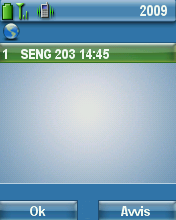
\includegraphics[scale=0.8]{alarmtelefon.png}
	\caption{Dagens skjermbilde}
	\label{gammelPasientsignal}
	\end{subfigure}
	\begin{subfigure}[b]{0.5\textwidth}
	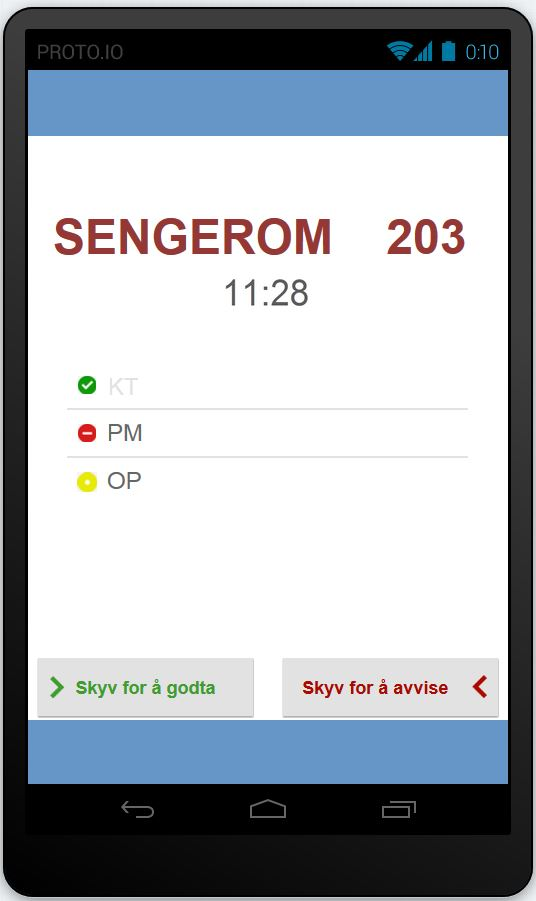
\includegraphics[scale=0.3]{proto_pasientsignal.jpg}
	\caption{Prototypens skjermbilde}
	\label{protoPasientsignal}
	\end{subfigure}
	\caption{Skjermbilde ved innkommende pasientsignal. Her fra sengerom 203.}
	\label{skjermbilder}
\end{figure}

\subsection{Statusindikator}
Statusindikatoren har som formål å fortelle hvilken status sykepleieren er satt til. Vi har valgt å bruke tre forskjellige statuser; $"$tilgjengelig$"$, $"$opptatt$"$ og $"$utilgjengelig$"$ (figur \ref{tilgjengelighetsstatuser}). Statusen vil i utgangspunktet være satt til $"$tilgjengelig$"$. Når en sykepleier går inn på et rom, vil dette som nevnt tilstedemarkere rommet, og sykepleierens status vil automatisk settes til $"$opptatt$"$. Når sykepleieren forlater rommet vil statusen igjen settes til $"$tilgjengelig$"$. Sykepleieren kan selv velge, uavhengig av lokasjon, å sette sin status til $"$utilgjengelig$"$. Denne statusen må manuelt settes tilbake til $"$tilgjengelig$"$ av sykepleieren.

\begin{figure}[H]
	\centering
	\begin{subfigure}[b]{0.3\textwidth}
		
\includegraphics[scale=0.15]{statusGronn.jpg}
		\caption{Tilgjengelig}
		\label{proto_startside}
	\end{subfigure}
	\begin{subfigure}[b]{0.3\textwidth}
		
\includegraphics[scale=0.15]{statusGul.jpg}
		\caption{Opptatt}
		\label{proto_startside}
	\end{subfigure}
	\begin{subfigure}[b]{0.3\textwidth}
		
\includegraphics[scale=0.15]{statusRod.jpg}
		\caption{Utilgjengelig}
		\label{proto_startside_medMeny}
	\end{subfigure}
	\caption{Tilgjengelighetsstatuser}
	\label{tilgjengelighetsstatuser}
\end{figure}

\subsection{Kontakter}
Kunnskap om kollegers tilgjengelighet kan også legges til grunn ved avgjørelser om, og hvordan man skal ta kontakt med andre sykepleiere. Dette skjermbildet viser kontaktinformasjon, inkludert tilgjengelighet til de sykepleierne som er på jobb. Dette kan gi en indikasjon på om en henvendelse til en kollega vil være forstyrrende. Ved å trykke på en av kontaktene vil man kunne velge om man vil ringe eller sende beskjed til denne.

\begin{figure}[H]
\centering
	\includegraphics[scale=0.3]{kontakter.jpg}
	\caption{Prototypens kontaktliste}
	\label{kontakter}
\end{figure}

\subsection{Øvrig funksjonalitet}
De øvrige funksjonene som her presenteres er inkludert av to grunner: (1) de skal gi prototypen en mer helhetlig fremtoning, og (2) representere mulighet for fremtidig funksjonalitet. Noen av disse er illustrert med skjermbilder.

\subsubsection{Forsiden}
Forsiden er illustrert i figur \ref{proto_startside}. Ikonet øverst til venstre gir tilgang til en drop-down meny som vist i figur \ref{proto_startside_medMeny}. 

\begin{figure}[H]
	\centering
	\begin{subfigure}[b]{0.48\textwidth}
		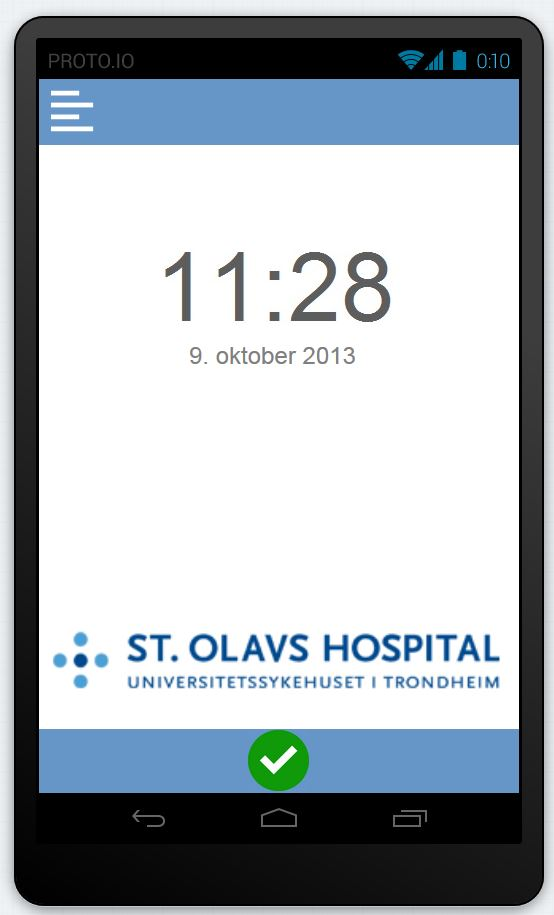
\includegraphics[scale=0.3]{proto_startside.jpg}
		\caption{Prototypens startside}
		\label{proto_startside}
	\end{subfigure}
	\begin{subfigure}[b]{0.48\textwidth}
		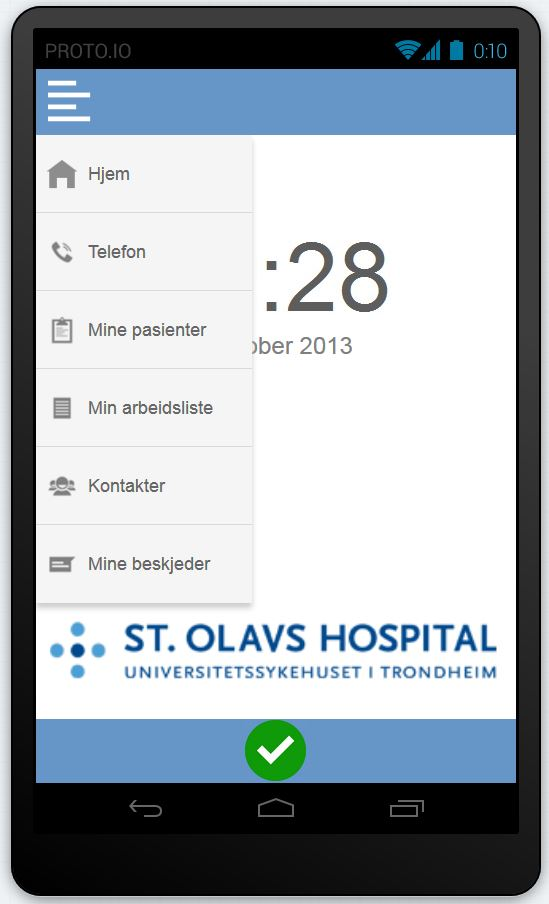
\includegraphics[scale=0.3]{proto_startside_medMeny.jpg}
		\caption{Prototypens startside med menyvisning}
		\label{proto_startside_medMeny}
	\end{subfigure}
	\caption{Prototypens startside}
\end{figure}

\noindent
Forsiden vises når skjermen slåes på. Vi har valgt kun klokke og datovisning i tillegg til status-indikatoren, for å begrense antall elementer på denne siden.

\subsubsection{Min Arbeidsliste}
Godtatte pasientsignaler legges i denne listen, og forsvinner når sykepleieren går inn på rommet hvor signalet ble utløst. Denne funksjonaliteten er allerede tilstede i dagens system.

\subsubsection{Mine Pasienter}
Dette er en oversikt over inneliggende pasienter, og vi ser for oss at det i fremtiden kunne være mulig å aksessere journaler, tidligere prøvesvar, samt få beskjed om endringer. Som vist i figur \ref{minePasienter} kan nye blodprøvesvar varsles og vises direkte på telefonen.

\begin{figure}[H]
\centering
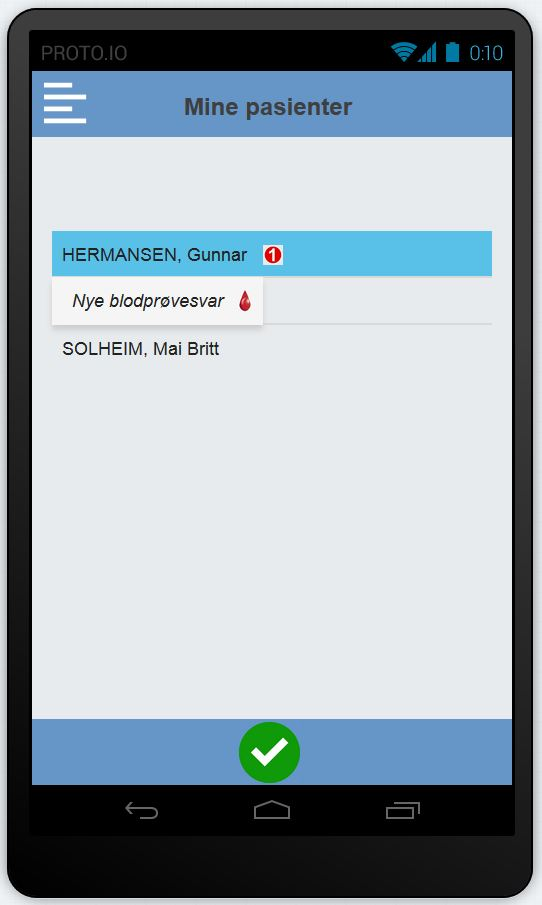
\includegraphics[scale=0.3]{minePasienter.jpg}
\caption{Eksempel på pasientlisten til en sykepleier. Her er det kommet svar på blodprøvende til Hermansen, (navnene på pasientene er fiktive).}
\label{minePasienter}
\end{figure}

\subsubsection{Mine Beskjeder}
Mine beskjeder er en sms-lignende tjeneste hvor sykepleierne kan stille hverandre spørsmål og gi beskjeder som ikke haster. Dette kan være en mindre forstyrrende måte å kommunisere på.

\subsubsection{Telefon}
Dette er vanlig telefonfunksjon.



